% =========================================================================
%        LaTeX Template for PhD Thesis
% =========================================================================

%\RequirePackage[l2tabu, orthodox]{nag} % display more warnings

\documentclass{sokendai_thesis} % for final version
%\documentclass[todo]{sokendai_thesis} % print todo notes (generated by this command: \mytodo[inline]{this is just a todo note})


% =====================================================
%  User-defined Commands
% =====================================================

\newcommand{\Order}{\mathit{O}} % for computational complexity


% =====================================================
%  Thesis Info
% =====================================================

\title{Latex Template for Sokendai Students}
\author{Taro Hitotsubashi}
\date{September 2015}
\crest{Crest/sokendai_crest.pdf} % comment out if you don't have a crest.
%\keywords{Latex Template, Sokendai, PhD Thesis} % for PDF meta-info


% =====================================================
%  Others
% =====================================================

% Typeset only specified chapters
%\includeonly{Manuscript/Introduction/introduction}


% =====================================================
%  Front Matter
% =====================================================

\begin{document}

\frontmatter
\maketitle

\listoftodos


\chapter*{Acknowledgments}

I would like to thank ...

\mytodo[inline]{Write Acknowledgments.}




\chapter*{Abstract}

This is a PhD thesis template for Sokendai students.
Use \textit{pdflatex} to build latex files.
This file specifies the following:
\begin{itemize}
	\item Font,
	\item Appearance of Text (Hyphenation and Letter-spacing),
	\item Page Layout,
	\item Theorem Environments,
	\item Header and Footer,
	\item Chapter Header,
	\item Table of Contents,
	\item Clickable PDF,
	\item Title Page and PDF-title.
\end{itemize}



\tableofcontents
\listoffigures
\listoftables
%% List of algorithms
%\listofalgorithms \addcontentsline{toc}{chapter}{List of Algorithms}

% =====================================================
%  Main Matter
% =====================================================

\mainmatter

\chapter{Introduction}\label{chapter:introduction}

\graphicspath{{Manuscript/Introduction/Figs/}}

This is a PhD thesis template for pdflatex.
Use \textit{pdflatex} to build latex files.
Don't use TeX+DVI (dvipdfm), or Microtype Package doesn't work.
If you write Japanese characters, use UTF-8 encoding. 

This file specifies the following items:
\begin{itemize}
	\item Font,
	\item Appearance of Text (Hyphenation and Letter-spacing),
	\item Page Layout,
	\item Theorem Environments,
	\item Header and Footer,
	\item Chapter Header,
	\item Table of Contents,
	\item Clickable PDF,
	\item Title Page and PDF-title.
\end{itemize}

The class file was made for Sokendai students.
If you are not a Sokendai student, rewrite the maketitle command in the class file.

We recommend to use \textit{TeX Live} to manage \LaTeX ~packages because this class file uses many packages. 
Before loading the class file, update all packages to the latest version using Tex Live.


%=========================================================================
\section{Managing todo items}
\makeatletter
\newcommand{\verbatimfont}[1]{\def\verbatim@font{#1}}%
\makeatother
\verbatimfont{\rmfamily}

You can make todo notes using the following command:
\begin{verbatim}
\mytodo[inline]{This is a inline todo note} 
\mytodo{This is a todo note at margin}.
\end{verbatim}

In order to display the todo items, use \textit{todo} option.
\begin{verbatim}
\documentclass[todo]{sokendai_thesis}
\end{verbatim}

If you do not want to display the items,
use the following command.
\begin{verbatim}
\documentclass{sokendai_thesis}
\end{verbatim}





\chapter{Tips} \label{chapter:tips}

\graphicspath{{Manuscript/Tips/Figs/}}

%=========================================================================
\section{English Writing}

% --------------------------
\subsection{Useful Sites}

\subsubsection{Springer Exemplar}
\url{http://www.springerexemplar.com/}

\subsubsection{Oxford Learner's Dictionaries}
\url{http://www.oxfordlearnersdictionaries.com}

\subsubsection{Thesaurus.com}
\url{http://www.thesaurus.com}


\subsection{Useful Books}

\begin{itemize}
	\item The Elements of Style, Fourth Edition~\cite{strunk1979}
\end{itemize}

%=========================================================================
\section{\LaTeX ~Tips}

% --------------------------
\subsection{Table} \label{sec:table}

Table~\ref{table:running_time} shows a sample.

\begin{table}[tbp]
% h:here, t:top, b:bottom, p:page of floats
\begin{center}
\begin{tabular}{c|ccc}
$n$  & Algorithm A  & Algorithm B & Ours  \\ \hline
20   & 100          & 150         & 10    \\
40   & 200          & 300         & 20    \\
60   & 400          & 600         & 30    \\
\end{tabular}
\caption{Running time}
\label{table:running_time}
\end{center}
\end{table}

% --------------------------
\subsection{Figure}

Figure~\ref{fig:graph} shows a sample.

\begin{figure}[tbp]
% h:here, t:top, b:bottom, p:page of floats
\begin{center} 
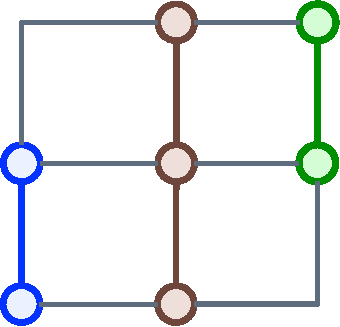
\includegraphics[width=3.5cm]{sample_graph.pdf}
\caption{Input graph}
\label{fig:graph}
\end{center} 
\end{figure}

% --------------------------
\subsection{Algorithm}

A sample from the manual of the algorithmicx package is shown in Algorithm~\ref{alg:euclid}.

\begin{algorithm}
\caption{Euclid's algorithm}\label{alg:euclid}
\begin{algorithmic}[1]
\Procedure{Euclid}{$a,b$}\Comment{The g.c.d. of $a$ and $b$}
   \State $r\gets a\bmod b$
   \While{$r\not=0$}\Comment{We have the answer if $r$ is 0}
      \State $a\gets b$
      \State $b\gets r$
      \State $r\gets a\bmod b$
   \EndWhile\label{euclidendwhile}
   \State \textbf{return} $b$\Comment{The gcd is $b$}
\EndProcedure
\end{algorithmic}
\end{algorithm}

\mytodo[inline]{Write more tips.}




\chapter{Sample}\label{chapter:sample}

\graphicspath{{Manuscript/Sample/Figs/}}

%=========================================================================
\section{About Sokendai}

\footnote{\url{http://www.soken.ac.jp/en/outline/message/}}
SOKENDAI (The Graduate University for Advanced Studies) was established in 1988 as Japan's first independent graduate university without undergraduate courses. SOKENDAI is unique in the world in that it provides comprehensive doctoral programs in academic fields ranging from the arts and humanities to science and engineering in cooperation with parent institutes, such as Inter-University Research Institutes, the excellent research and learning environments of which are fully leveraged to nurture leading researchers with outstanding expertise and broad perspectives.

All students enrolled in SOKENDAI are from other national, public, and private universities (new students enrolled in academic year 2014 are from 64 universities, including 15 overseas universities). One of the greatest disadvantages of higher education in Japan resides in its low fluidity, which results in unilinearity and sectionalism. However, students admitted to SOKENDAI are already free of the negative effects thereof. Therefore, the remarkable potential of SOKENDAI students is backed by their own experience of successfully leaping over numerous barriers; many of them are also endowed with the guts and ability to take on challenges across the boundaries of fields and academic disciplines. This is one of the characteristics of SOKENDAI that has most benefited the University and individual students. In fact, new encounters with people and contact with new academic cultures give us great power to develop new knowledge.

The second characteristic of SOKENDAI is that graduate education is conducted in an excellent environment, more specifically, at the front lines of study at the affiliated 18 Inter-University Research Institutes. These parent Institutes have top-ranking research personnel who diligently collaborate with researchers from Japan and overseas, as well as the world's most sophisticated research equipment, facilities, materials, and databases. The Institutes promote highly specialized international research activities and interdisciplinary joint studies with researchers from universities/research institutes across Japan and other countries. Thus, SOKENDAI can aim at nurturing researchers with ``high expertise'', ``international competency'', and ``cross-disciplinary cooperativeness''.

The third characteristic of SOKENDAI is its systematic and organizational approach to encouraging students to acquire ``comprehensive ability'' in addition to high expertise. Across the parent institutes and the departments of SOKENDAI, research activities are in progress in a wide variety of fields, including culture, history, information, life, human physiology, energy, material, and space. Students here can make good use of this academic diversity to obtain the ``broad perspective'' necessary for situating their own expertise in the whole of knowledge, one aspect of the acquisition of comprehensive ability. New academic disciplines often straddle the boundaries between fields and develop with the input of researchers from different fields. Since the knowledge required for such new areas of study cannot be framed within the limits of individual departments or schools, it is necessary to provide interdisciplinary education across multiple departments or schools. In order to tackle this need, SOKENDAI has been promoting ``interdepartmental programs''. SOKENDAI students can obtain ``cross-disciplinary competence'' through education across departments/schools and joint learning/research activities rooted in interdisciplinary cooperation. This is the second aspect of the acquisition of comprehensive ability. Nowadays, many of the fruits of science have already been materialized in society and are making an impact on people's lives. Scientists are required to be accountable for the results of their research and even the outcomes arising from the application of these results. In other words, modern scientists need to master the comprehensive ability as individuals taking into account humankind and society. The third aspect of the acquisition of the comprehensive ability is that SOKENDAI strives to attain the ideal of ``science linked with society''.

The objectives of SOKENDAI are: (i) to nurture international researchers with high expertise and broad perspectives as well as an understanding of cross-disciplinary cooperation and social relationships; (ii) to proceed with interdisciplinary, pioneering and expansive research on the basis of the linkage between the parent institutes and the Hayama Campus and through collaboration with Japanese and international researchers, and; (iii) to establish its position as a hub for graduate education in Asia for the creation of science linked with society.

It is my hope that SOKENDAI students gain a good understanding of these characteristics and objectives of the University and take on challenging research subjects while making full use of the resources provided. Although graduate students have a lot to do in their everyday learning and research activities, I also hope that they make efforts to develop relationships with those who specialize in different academic fields or come from different universities and countries. Human connections obtained through such efforts will surely yield great rewards in their future research lives. In addition, Japanese students are encouraged to master foreign languages, and international students the Japanese language. As in the case of interaction among multiple areas of expertise, so to be proficient in intercultural communication is a prerequisite for exercising one's ability as a doctoral level researcher equipped with international competency. SOKENDAI also strives to promote multilingualism in the education of students.

We, the faculty and staff of SOKENDAI, will consistently work with our students to further evolve the University's characteristics and to achieve our objectives. In this regard, we ask all concerned to understand and cooperate in the further development of SOKENDAI.

April 1, 2015

%=========================================================================
\section{Lorem Ipsum}

%\kant
%\lipsum


%
%\blindtext
%\Blindtext
%
%\blinditemize
%\blindenumerate
%\blinddescription
%
%\blindmathtrue
%\blindmathfalse
%
\blindmathpaper
%
%\blinddocument
%\Blinddocument




% =====================================================
%  Back Matter
% =====================================================

%\backmatter


% =====================================================
%  Bibliography
% =====================================================

%\bibliographystyle{plain}
\bibliographystyle{unsrt}
\bibliography{Bib/reference}


% =====================================================
%  Appendices
% =====================================================

\begin{appendices}

%\chapter{Tips} \label{chapter:tips}

\graphicspath{{Manuscript/Tips/Figs/}}

%=========================================================================
\section{English Writing}

% --------------------------
\subsection{Useful Sites}

\subsubsection{Springer Exemplar}
\url{http://www.springerexemplar.com/}

\subsubsection{Oxford Learner's Dictionaries}
\url{http://www.oxfordlearnersdictionaries.com}

\subsubsection{Thesaurus.com}
\url{http://www.thesaurus.com}


\subsection{Useful Books}

\begin{itemize}
	\item The Elements of Style, Fourth Edition~\cite{strunk1979}
\end{itemize}

%=========================================================================
\section{\LaTeX ~Tips}

% --------------------------
\subsection{Table} \label{sec:table}

Table~\ref{table:running_time} shows a sample.

\begin{table}[tbp]
% h:here, t:top, b:bottom, p:page of floats
\begin{center}
\begin{tabular}{c|ccc}
$n$  & Algorithm A  & Algorithm B & Ours  \\ \hline
20   & 100          & 150         & 10    \\
40   & 200          & 300         & 20    \\
60   & 400          & 600         & 30    \\
\end{tabular}
\caption{Running time}
\label{table:running_time}
\end{center}
\end{table}

% --------------------------
\subsection{Figure}

Figure~\ref{fig:graph} shows a sample.

\begin{figure}[tbp]
% h:here, t:top, b:bottom, p:page of floats
\begin{center} 
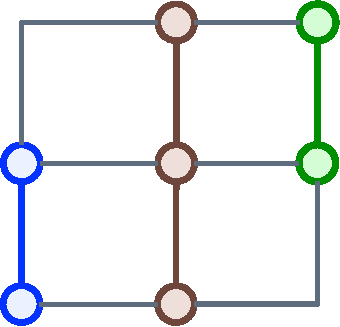
\includegraphics[width=3.5cm]{sample_graph.pdf}
\caption{Input graph}
\label{fig:graph}
\end{center} 
\end{figure}

% --------------------------
\subsection{Algorithm}

A sample from the manual of the algorithmicx package is shown in Algorithm~\ref{alg:euclid}.

\begin{algorithm}
\caption{Euclid's algorithm}\label{alg:euclid}
\begin{algorithmic}[1]
\Procedure{Euclid}{$a,b$}\Comment{The g.c.d. of $a$ and $b$}
   \State $r\gets a\bmod b$
   \While{$r\not=0$}\Comment{We have the answer if $r$ is 0}
      \State $a\gets b$
      \State $b\gets r$
      \State $r\gets a\bmod b$
   \EndWhile\label{euclidendwhile}
   \State \textbf{return} $b$\Comment{The gcd is $b$}
\EndProcedure
\end{algorithmic}
\end{algorithm}

\mytodo[inline]{Write more tips.}





\end{appendices}


\end{document}
